\documentclass[11pt,a4paper,twoside]{article}

% You should not change the line above.
% Nor change any of the formating.

% At a minimum, you need to edit the preamble file for your name and project
% title. There are a lot of latex commands there you might find useful.
\usepackage[a4paper]{geometry}
\usepackage{amsfonts}
\usepackage{amsthm}
\usepackage{amsmath}
\usepackage{parskip}
\usepackage{mathrsfs}
\usepackage{graphicx}
\usepackage{amssymb}
\usepackage{xtab}

% You need to set the next two items. 
% If you title is long, you may need to adjust the spacing in titlepage.tex
\newcommand{\TheAuthor}{Your Name}
\newcommand{\TheTitle}{Your Project title}

% uncomment exacly one of these
\newcommand{\TheModule}{\bf MA4K8 Scholarly Report}
%\newcommand{\TheModule}{\bf MA4K9 Dissertation}


% Leave the following two as is
\newcommand{\TheUni}{The University of Warwick}
\newcommand{\TheDept}{Mathematics Institute}

% Set the correct submission year, e.g. replace 2000 with 2017
\newcommand{\TheSubDate}{\monthyear \formatdate{5}{4}{2000}}

% The are a lot of things you might find useful and want to uncomment. 
% Most things you will want to uncomment or change will be near the top.

% standard maths symbols (you probably want to uncomment all of these)
% \newcommand{\Z}{\ensuremath{\mathbb{Z}}}% integers
% \newcommand{\N}{\ensuremath{\mathbb{N}}}% natural numbers
% \newcommand{\R}{\ensuremath{\mathbb{R}}}% real numbers
% \newcommand{\C}{\ensuremath{\mathbb{C}}}% complex numbers

% Others 
%\newcommand{\st}{\ensuremath{:}}% such that
%\newcommand{\Tau}{\ensuremath{\mathcal{T}}}
%\newcommand{\Nat}{\mathbb{N}}

%\usepackage[numbers]{natbib}% round braces, sort multiple citations
%\usepackage{hyperref}% creates hypertext links in pdf files (natbib compatible)
\usepackage{setspace}
%\usepackage{fancyhdr}
%\usepackage{mathrsfs}
%\usepackage{textcomp}
%\usepackage{color}
%\usepackage{graphicx}
%\usepackage{framed}
% \usepackage{algorithmic}% format pseudocode
%\usepackage[vlined,boxed,commentsnumbered,algochapter]{algorithm2e}
% \usepackage[chapter]{algorithm}% float wrapper for algorithms
%\usepackage{amsmath}% American Mathematical Society macros - essential!
%\usepackage{amssymb}% contains amsfonts
%\usepackage{amsthm}% allows more flexibility with theorems
\usepackage[nodayofweek]{datetime} % change the format of printed dates (no american style!) 
%\usepackage{ifdraft}% perform operations conditional on the draft option

% \usepackage{mathptmx}
% \usepackage{mathpazo}
%\usepackage{amscd}
% \usepackage{xy}
% \usepackage{diagxy}
%\usepackage{diagrams}

%\usepackage{marginnote}
%\usepackage{rotating}
%\usepackage{multirow}
% \usepackage{polski}
% \usepackage[T1]{fontenc}
% \usepackage{tikzpicture}
% \usetikzlibrary{matrix,arrows}

% \usepackage[inline]{showlabels}
%\usepackage{booktabs}

% Date format

% Use the datetime package
\newdateformat{monthyear}{\monthname[\THEMONTH], \THEYEAR}% new date format

% New commands, operators and symbols

% Operators
%\DeclareMathOperator{\Sym}{Sym}% symmetric group
%\DeclareMathOperator{\Alt}{Alt}% alternating group
%\DeclareMathOperator{\Id}{Id}
%\DeclareMathOperator{\Hom}{Hom}
%\DeclareMathOperator{\Grp}{Grp}
%\DeclareMathOperator{\supp}{supp}
%\DeclareMathOperator{\fix}{fix}
%\DeclareMathOperator{\dep}{dep}
%\DeclareMathOperator{\lcm}{lcm}
%\DeclareMathOperator{\Aut}{Aut}
%\DeclareMathOperator{\Inn}{Inn}
%\DeclareMathOperator{\Out}{Out}
% \DeclareMathOperator{\dim}{dim}
%\DeclareMathOperator{\Syl}{Syl}
%\DeclareMathOperator{\Hall}{Hall}
%\DeclareMathOperator{\pCore}{pCore}
%\DeclareMathOperator{\Char}{char}
%\DeclareMathOperator{\Image}{Im}
%\DeclareMathOperator{\Ker}{Ker}
%\DeclareMathOperator{\Hcf}{hcf}
%\DeclareMathOperator{\GL}{GL}
%\DeclareMathOperator{\Pc}{Pc}
%\DeclareMathOperator{\Stab}{Stab}
%\DeclareMathOperator{\Orbit}{Orbit}


% Hyphenation fixes
%\newcommand{\letdash}[1]{$#1$\nobreakdash-\hspace{0pt}}% for n-element, k-transitive etc
%\newcommand{\numdash}{\nobreakdash--}

% Sequences
%\newcommand{\seqfin}[3]{\ensuremath{#1_{#2}, \dotsc , #1_{#3}}}
%\newcommand{\seqinf}[3]{\ensuremath{#1_{#2}, #1_{#3}, \dotsc}}

% New environments

% Dedication
%\newenvironment{dedication}
%{\clearpage \thispagestyle{empty} \vspace*{\stretch{1}} \begin{center} \em}
%{\end{center} \vspace*{\stretch{3}} \clearpage}


% Page Layout

% Dimensions
% Use the geometry package to set this up
\geometry{includehead,includefoot,left=3cm,right=3cm,top=2cm,bottom=2cm}% head and foot are included in total body so that nothing is printed out of the boundaries of the set margins

% Header and footer
% Use the fancydr package
%\ifdraft{%
%\fancypagestyle{plain}{% redefine plain pagestyle for draft
%\renewcommand{\headrulewidth}{0pt}% no head rule in draft mode
%\fancyhf{}% clear headers and footers
%\fancyhead[C]{\ifdraft{DRAFT}{}}% print DRAFT across top if the draft option is set
%\fancyfoot[C]{\thepage}% usual page numbering
%

%\pagestyle{fancy}
%\renewcommand{\chaptermark}[1]{\markboth{\thechapter.\ #1}{}}% compact with no capitalisation
%\renewcommand{\sectionmark}[1]{\markright{\thesection.\ #1}}% compact with no capitalisation
%\ifdraft{\renewcommand{\headrulewidth}{0pt}}{}% no head rule in draft mode
%\setlength{\headheight}{15pt}
%\fancyhf{}% clear all header and footer fields
% one-sided printing, so no E,O distinction need be made
%\fancyhead[C]{\ifdraft{DRAFT}{}}% print DRAFT across top if the draft option is set
%\fancyhead[R]{\thepage}% page in top right
%\fancyhead[L]{\ifdraft{}{\leftmark}}% chapter number and title in top left

% Theorems
%
%\newtheorem{prop}{Proposition}[chapter]
%\newtheorem{lemma}[prop]{Lemma}
%\newtheorem{conjecture}[prop]{Conjecture}
%\newtheorem{theorem}[prop]{Theorem}
%\newtheorem{hyp}[prop]{Hypothesis}
%\newtheorem{cor}[prop]{Corollary}
%\newtheorem{claim}[prop]{Claim}
%\newtheorem{remark}[prop]{Remark}
%\newtheorem{notation}[prop]{Notation}
%\newtheorem{defn}[prop]{Definition}


% Numbering
%\numberwithin{equation}{chapter}% standard style numbering, nothing special here


% Algorithms

% Use the algorithms package.
% \renewcommand{\algorithmicrequire}{\textbf{Input:}}
% \renewcommand{\algorithmicensure}{\textbf{Output:}}
% \renewcommand{\algorithmiccomment}[1]{/* #1 */}
%\RestyleAlgo{boxruled}
%\SetAlgoInsideSkip{medskip}
%\setlength{\algomargin}{2em}
%\setlength{\interspacetitleboxruled}{0.7em}
%\setlength{\interspacetitleruled}{0.7em}
%\LinesNumbered
%\SetAlCapNameSty{sc}
%\SetFuncSty{sc}

%\newenvironment{spacedalgorithm}{\begin{algorithm}\onehalfspacing}{\end{algorithm}}
% \newenvironment{onehalfverbatim}{\onehalfspacing\begin{verbatim}}{\end{verbatim}}

%\reversemarginpar
%\newcounter{nootje}
%\setcounter{nootje}{1}
%\renewcommand\check[1]{[*\thenootje]\marginnote{\tiny\begin{minipage}{40mm}\begin{flushright}\thenootje
%: #1\end{flushright}\end{minipage}}\addtocounter{nootje}{1}}


% Document details



\begin{document}

\pagenumbering{roman}
\begin{titlepage}
\begin{center}

\includegraphics[width=5cm]{Warwick_Crest} 
% this graphic file should live in the working directory
% the size of the following arguments to vspace were determined by 
% trial and error, and produce suitable output for the A4 pagesize.

\vspace*{20pt}
\begin{spacing}{2}
\begin{center}
{\Large \bf \TheTitle} % declared in preamble.tex

\vspace*{14pt}

by

{\Large \bf \TheAuthor} % declared in preamble.tex

\vspace*{16pt}

{\large \bf \TheModule} % declared in preamble.tex


Submitted to \TheUni % declared in preamble.tex

\vspace*{36pt}
{\Large \bf \TheDept} % declared in preamble.tex

\TheSubDate % declared in preamble.tex

\vspace*{36pt}

\includegraphics[width=5cm]{warwick_logo} 
% this graphic file should live in the working directory

\end{center}
\end{spacing}
\end{center}
\end{titlepage}

\setcounter{page}{2}
%\renewcommand{\contentsname}{Table of contents}
\tableofcontents
\cleardoublepage
\onehalfspacing
\pagenumbering{arabic}
\onehalfspacing
\raggedbottom

% Now starts the main part of the report. 
% Each section/chapter is in a separate file. Two examples are include.
% 
% This part (between TOC and Bibliograpy) must obey:
% for MA4K8 must not exceed 30 pages.
% for MA4K9 the target is approx 30 pages and must not exceed 40 pages.

\section{Introduction}

Consider a PDE of the following form:

\begin{align*}
    \partial_t u = N(u)\\
\end{align*}

These PDEs of this from are common when looking into Phase boundary problems such as the Allen-Cahn equations. %maybe add a citation
While for some instances exact soltions to these PDEs exist and are known, in many practical cases however it is often neccessary to compute approximate solutions to these PDEs.
In order to achieve this, we will need to discretise in space yielding an ODE.
We do this via finite element methods giving:
\begin{align*}
    M\frac d{dt} u_h = N_h(u)\\
\end{align*}
For a mass matrix $M$ and some $N_h$.
From here we can apply methods that can solve this ODE in time.


\section{Solution Schemes} \label{section:methods}
Now, we outline the methods by which the ODEs arising from the discretization of PDEs in space can be solved. 
Consider the following PDE:
\begin{align*}
    \dot u_t &= N(u)
\end{align*}
Discretizing in space gives the following:
\begin{align*}
M\dot u_h(t) &= N_h(u_h(t))\\ %\text{ where $M$ is the mass matrix}
\text{using } R(u_h(t)) &= N_h(u_h(t)) - DN(u_h(t))u_h(t) \text{ to denote the non-linear term gives}\\
M\dot u_h(t) &= DN(u_h(t))u_h(t) + R(u_h(t))\\
\dot u_h(t) &= M^{-1}(DN(u_h(t))u_h(t) + R(u_h(t)))
\end{align*}
\subsection{Methods}
We present both conventional ODE solvers such as the forwards and backwards Euler method before moving on to the exponential integrator methods.
For a time step $\tau$ we compute $u_h(t+\tau)$ in the following ways: 

\subsubsection{Forwards Euler}
The forwards Euler method is given by:
\begin{align*}
u_h(t+\tau) = u_h(t) + \tau M^{-1}N_h(u_h(t))
\end{align*}

\subsubsection{Backwards Euler}
The backwards Euler method is given by:
\begin{align*}
u_h(t+\tau) = u_h(t) + \tau M^{-1}N_h(u_h(t+\tau))
\end{align*}
As this method is implicit, we will need to employ a Newton solver.

\subsubsection{Explicit Exponential Scheme} %check this is correct%
For the explicit exponential integrator schemes we use the following formula:
\begin{align*}
u_h(t+\tau) &= e^{\tau M^{-1} DN(u_h(t))}(u_h(t) + M^{-1}R(u_h(t)))
\end{align*}


\subsubsection{First Order Exponential Integrator}
Here, we also present another integrator from Huang Et al \cite{Huang2022}
\begin{align*}
u_h(t+\tau) &= e^{\tau M^{-1} DN(u_h(t))}u_h(t) + \tau \varphi_1(\tau M^{-1} DN(u_h(t)))R(u_h(t))
\end{align*}
Where:
\begin{align*}
    \varphi_k(z) &= \int^1_0e^{(1-\theta)z}\frac{\theta^{k-1}}{(k-1)!}d\theta, k \geq 1
\end{align*}

\subsubsection{Second Order Exponential Integrator}
We also look at a second order exponential integrator \cite{Huang2022}.
\begin{align*}
    \text{writing } A &= \tau M^{-1} DN(u_h(t)) \text{ for the sake of brevity}\\
    u_h(t+\tau) &= e^{A}u_h(t) + \tau((\varphi_1(A)) - \frac 1{c}\varphi_2(A))R(u_h(t))\\
    & + \frac1{c}\varphi_2(A)R(e^{cA}u_h(t) + c\tau\varphi_1(c A)R(u_h(t)))
\end{align*}
where $c \in (0,1]$.

\subsection{Mass Matrix}
When using these schemes it is necessary to be able to compute the inverse mass matrix $M^{-1}$.
Attempting to compute the exact inverse can be computationally intensive. While for a fixed spacial discretization this may be acceptable, as it will only need to be computed once, for an adaptive grid this may be impractical.
As a result, we employ mass lumping where each row is summed up and placed on the diagonal of the matrix.
From here, computing the inverse is straightforward.

\section{Numerical Experiments}

\subsection{Travelling Wave Allen Cahn}
In this section we run numerical experiments compairing the backward Euler method to Krylov methods for computing solutions to a PDE.
Specifically we will investigate the initial boundary value problem for the Allen Cahn equation on a strip with a traveling wave solution\cite{YukitakaFukao2004} given by:

\begin{align}
    \hat u(x,y,t)&=\frac{e^{\frac{x-ct}{\sqrt2}}}{1+e^{\frac{x-ct}{\sqrt2}}} \label{TravelingWaveSol}\\
    \text{where } c &= \frac{\sqrt{2}}{4}
\end{align}
and where the problem is defined as follows:
\begin{align*}
    u_t&=\Delta u+u(u-\frac14)(1-u) \text{ on $\Omega \times [0, 8]$}\\
    \text{with } \Omega &= \mathbb{R}\times[-1,1]\\
    \nabla u \cdot \hat n &= g \text{ for $g = \nabla \hat u \cdot \hat n$}\\
    u_0(x, y) &= \hat u(x,y, 0)
\end{align*}
However for our numerical experiments we compute on the space $\Omega=[-16,16]\times[-1,1]$.
Where $u$ is the solution, we write it in weak form.
\begin{align*}
    \dot u&=\Delta u+u(u-\frac14)(1-u)\\
    \int_{\Omega} \dot u v &=\int_{\Omega} \Delta uv+u(u-\frac14)(1-u)v \text{ for a smooth function $v \in C^{\infty}(\overline{\Omega})$}\\
    \int_{\Omega} \dot u v &=\int_{\Omega} u(u-\frac14)(1-u)v - \nabla u \cdot \nabla v + \int_{\partial\Omega}  v\hat n \cdot \nabla u\\
    \text{subsituting in } u_h(t,x,y) &= \sum_i u_i(t) v_i(x,y) \text{ where $(v_i)$ are the test functions we obtain:}\\
    \text{we get } \sum_i\int_{\Omega} \dot u_i v_i v_j &=\sum_i(\int_{\Omega} u_iv_i(u_iv_i-\frac14)(1-u_iv_i)v_j - \int_{\Omega}\nabla (u_iv_i) \cdot \nabla v_j + \int_{\partial\Omega}  v_j\hat n \cdot \nabla \hat u_iv_i)\\
    \sum_iu_i\int_{\Omega}v_iv_j &= -u_i\sum_i(\int_{\Omega}\nabla v_i \cdot \nabla v_j + \int_{\Omega}R(u_h)v_j)\\
    \text{where we have } R(u)&=u(u-\frac14)(1-u) + \int_{\partial\Omega}  \hat n \cdot \nabla \hat  u\\
    \intertext{The above is true for all $i=0,1,2,...,n$. Writing in matrix vector form gives}
    M \underline{\dot u} &= DN(\underline{u})\underline{u} + R(\underline{u})\\
    \text{where } M_{i,j} &= \int_{\Omega}v_iv_jdx
\end{align*}
In the tests, we will investigate the relation between step size, $L_2$ error given by $||\hat u - \underline{u}||_{L_2}$ and call to the operator $N$ which will be a crude approximation to the computational cost.
We compare the Backward Euler, First and Second order expoenntial methods over grid sizes: $128 \times 8$ and $256 \times 8$ and with time step $\tau=8,4,2,1,0.5,0.25,0.125,0.0625,0.03125$.

\subsubsection{Experimental Results}

Bellow we show the $L_2$ error with respect to the time step $\tau$.
Where in the legend EXP1LAN 16 denotes the first order method with Krylov size 16, likewise for EXP2LAN and the second order method.
BE denotes the backwards Euler method.

\begin{figure}[H]
    \centering
    \begin{minipage}{0.49\textwidth}
        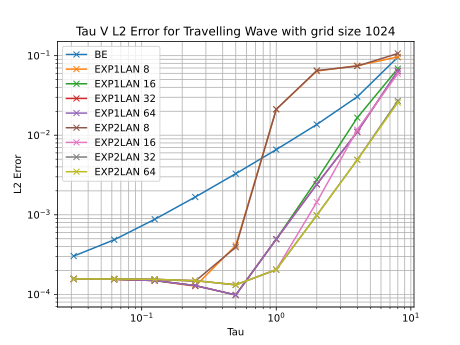
\includegraphics[width=1\textwidth]{Graphs/TravellingWave/Tau V L2 Error for Travelling Wave with grid size 1024.png} % Change filename to your image
        \caption{$\tau$ vs $L_2$ with grid size 1024}
        \label{fig:plot1}
    \end{minipage}\hfill
    \centering
    \begin{minipage}{0.49\textwidth}
        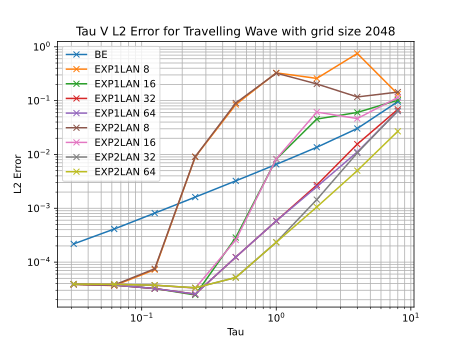
\includegraphics[width=1\textwidth]{Graphs/TravellingWave/Tau V L2 Error for Travelling Wave with grid size 2048.png} % Change filename to your image
        \caption{$\tau$ vs $L_2$ with grid size 2048}
        \label{fig:plot2}
    \end{minipage}\hfill
\end{figure}

First see that all of the methods tested converge, tending towards the discritisation error.
The discritisation error is smaller on the more detailed grid.
The Krylov methods converge faster than the backwards Euler method.
We notice that when a smaller Krylov subspace is used that the expoenntial methods only start to converge for a sufficiently small $\tau$.
Likewise when these methods start to converge we observe that they perform simillarly to the methods using a larger subspace, however they will require fewer operator calls.
This suggests that for sufficient small time steps a shallower subspace may suffice.
Likewise for the converse that larger timesteps require a deeper krylov subspace.

Now we compare the error with the number of calls to the operator.
These operator calls are needed for computing $N$ which is used with the matrix free methods as described above as well as for computing the non-linear term $R$.

\begin{figure}[H]
    \centering
    \begin{minipage}{0.49\textwidth}
        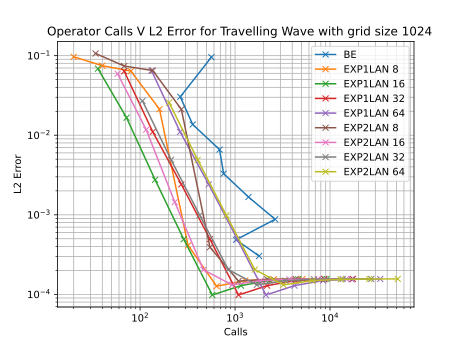
\includegraphics[width=1\textwidth]{Graphs/TravellingWave/Operator Calls V Error for Travelling Wave with grid size 1024.png} % Change filename to your image
        \caption{$\tau$ vs $L_2$ with grid size 1024}
        \label{fig:plot1}
    \end{minipage}\hfill
    \centering
    \begin{minipage}{0.49\textwidth}
        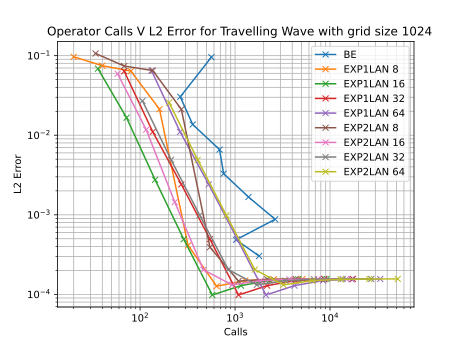
\includegraphics[width=1\textwidth]{Graphs/TravellingWave/Operator Calls V Error for Travelling Wave with grid size 1024.png} % Change filename to your image
        \caption{$\tau$ vs $L_2$ with grid size 2048}
        \label{fig:plot2}
    \end{minipage}\hfill
\end{figure}

We see that as expected that when a larger Krylov subspace is used that more calls to the operator are required.
We also observe that the exponential methods outperform the BE by achieving a lower error with fewer calls to the operator.

Here we present the experimental orders of convergence for the grid size 1024.

\begin{table}[H]
    \centering
    \begin{tabular}{| c | c | c | c}
    \hline
    BE & EXP1LAN 64 & EXP2LAN 64 \\
    \hline
    1.656175178817219 & 2.5200121901844423 & 2.427488988868435 \\
    1.159963039219372 & 2.147211103525317 & 2.2448741639287576 \\
    1.0543798412512431 & 2.1084233436748687 & 2.175268892119002 \\
    1.0188791686457326 & 2.235535140373336 & 2.176237872787299 \\
    1.0016513655730614 & 2.2847781778148475 & 0.6355415381730404 \\
    0.9874831778164389 & -0.3463812590562603 & -0.1610890501147955 \\
    0.9808216274859436 & -0.2097197508087928 & -0.0545528584432596 \\
    0.919336864575657 & -0.051644372942987 & -0.01407844052927163 \\
    \hline
    \end{tabular}
    \caption{Experimental orders of convergence}
    \label{tab:EOCs}
\end{table}


We observe that the rate of convergence for the second order method was inline with what has been shown analytic\cite{Huang2022} at a rate of $2$.
The first order method converges with a rate of 2 despite an expectation of a rate of $1$\cite{Huang2022}.
The exponential methods stop converging as they reach the discritisation error.
The backwards euler converges at the rate expceted of 1.

\subsection{A 2D Allen Cahn Problem}

We will now look into the two dimentional Allen Cahn Problem given by:
\begin{align*}
    u_t &= -\Delta u + u (u^2-1) \text{ } \Omega=[0,1]\times[0,1]
\end{align*}
With Neumann boundary conditions.
The initial condition is chosen by randomly setting points on the grid from a uniform distribution in the range $-0.9,0.9$.
The same randomly generated initial condition will be used for each test.
As we do not have an exact solution, we will use the backwards Euler method with a timestep of $\tau = 10^{-4}$ to genarate a referance solution.
We will compare the backwards Euler method to the first and second order expoenntial integrator methods described above.
The tests are run on a $60\times60$ grid with the end time being $t_e=24$.
The error is computed by calculating the $L_2$ error between the prediction of the chosen stepper and the reference solution. 
Below we present our results.

\subsubsection{Experimental Results}

We begin by compairing the timestep size $\tau$ to the $L_2$ error for the different methods.

\begin{figure}[H]
    \centering
    \begin{minipage}{0.49\textwidth}
        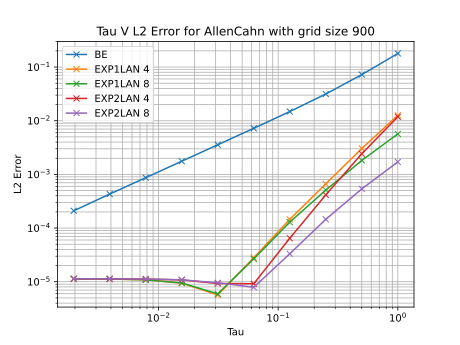
\includegraphics[width=1\textwidth]{Graphs/AllenCahn/Tau V L2 Error for AllenCahn with grid size 900.png} % Change filename to your image
        \caption{$\tau$ vs $L_2$ with grid size 900}
        \label{fig:ACtauE}
    \end{minipage}\hfill
    \centering
    \begin{minipage}{0.49\textwidth}
        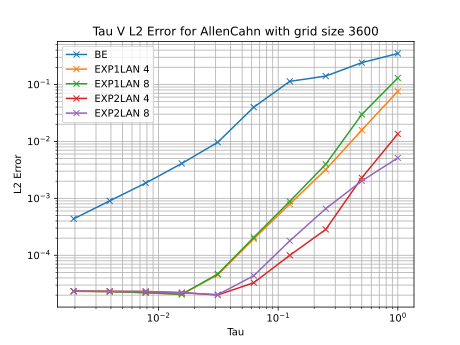
\includegraphics[width=1\textwidth]{Graphs/AllenCahn/Tau V L2 Error for AllenCahn with grid size 3600.png} % Change filename to your image
        \caption{$\tau$ vs $L_2$ with grid size 3600}
        \label{fig:ACtauE1024}
    \end{minipage}\hfill
\end{figure}

We observe convergence in both expoential methods for both krylov sizes.
These methods significantly outperform the backwards Euler method, simillar to the traveling wave Allen Cahn problem given above.
For this problem a relatively shallow subspace has been used compaired to above and appears to be sufficient.

Below as before we present the number of calls to the operator against the error.
\begin{figure}[H]
    \centering
    \begin{minipage}{0.49\textwidth}
        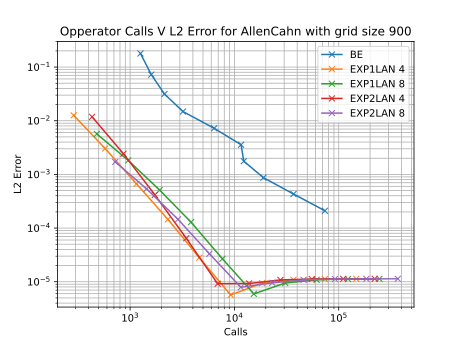
\includegraphics[width=1\textwidth]{Graphs/AllenCahn/Operator Calls V Error for AllenCahn with grid size 900.png} % Change filename to your image
        \caption{Operator calls vs $L_2$ with grid size 900}
        \label{fig:plot1}
    \end{minipage}\hfill
    \centering
    \begin{minipage}{0.49\textwidth}
        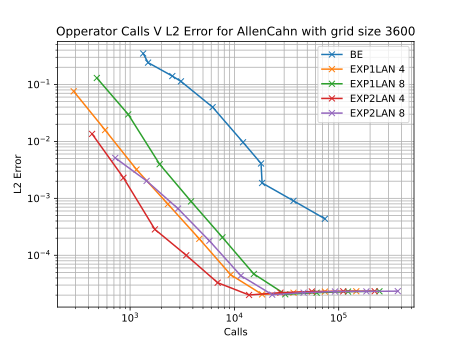
\includegraphics[width=1\textwidth]{Graphs/AllenCahn/Operator Calls V Error for AllenCahn with grid size 3600.png} % Change filename to your image
        \caption{Operator calls vs $L_2$ with grid size 3600}
        \label{fig:plot2}
    \end{minipage}\hfill
\end{figure}
For both methods we see that to achive a lower error requires more calls to the operator.
We see that in terms of performance the backwards Euler method performs significantly worse in comparison to both of the expoential methods.

Here we present the experimental orders of convergence on a grid size of 3600.

\begin{table}[H]
    \centering
    \begin{tabular}{| c | c | c |}
    \hline
    BE & EXP1LAN 8 & EXP2LAN 8 \\
    \hline
    0.5336772856567727 & 2.124425468811078    & 1.3416905476319223 \\
    0.7835756762460372 & 2.905742997002231    & 1.6172444544625373 \\
    0.3087677833100485 & 2.1667343028183392   & 1.8766417619133886 \\
    1.504631886802277  & 2.0994616006682154   & 2.034301870712038 \\
    2.0486348034911237 & 2.13577903687606     & 1.1061518243743675 \\
    1.237052619854426  & 1.184386408121027    & -0.11660694297267732 \\
    1.1376542802507796 & -0.09373274955254216 & -0.06785678855256895 \\
    1.0396362359013922 & -0.06516215516412459 & -0.005698148120031917 \\
    1.0482179972577244 & -0.01797864948877803 & -0.01442779444997218 \\
    \hline
    \end{tabular}
    \caption{Experimental orders of convergence}
    \label{tab:reduced_data}
\end{table}

Again we observe first order convergence for the backwards Euler methods and second order convergence for the two exponential integrator methods.

\subsection{Reaction Diffusion}

For both of the above problems the first order exponential method converged with rate 2.
In order to verify correct implementation, and to be able to compare the backwards Euler method to the first order expoenential method in a "fairer" way we study the following reaction diffusion problem\cite{Huang2022}.

\begin{align*}
    u_t &= -\frac12\Delta u + \frac12 \pi^2u + \frac12 \pi^2 e^{-\pi^2t}sin(\pi x)sin(\pi y) \text{ } (x,y)\in\Omega t\in\times[0,t_e]\\
    u(0,x,y) &= (sin(\pi x) - 1)sin(\pi y) \text{ } (x,y)\in \Omega
\end{align*}

With the following exact solution:

\begin{align*}
    u(t, x, y) &= e^{-\pi^2t}(sin(\pi x) - 1)sin(\pi y)
\end{align*}

With homogenous Dirichlet boundary conditions.
Where $\Omega = (\frac12, \frac52)\times(0,1)$ and our end time is given by $t_e = 0.1$.
We run our tests on grid sizes of $128\times64$ and $256\times128$ and use times steps sizes of $\tau=\frac{0.1}{2^i}$ for $i = 0,1,...,4$


We begin by compairing the timestep size $\tau$ to the $L_2$ error for the different methods.
\begin{figure}[H]
    \centering
    \begin{minipage}{0.49\textwidth}
        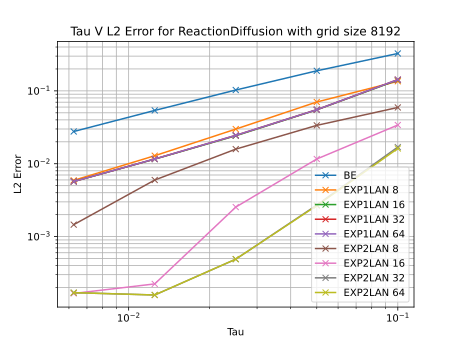
\includegraphics[width=1\textwidth]{Graphs/ReactionDiffusion/Tau V L2 Error for ReactionDiffusion with grid size 8192.png} % Change filename to your image
        \caption{$\tau$ vs $L_2$ with grid size 8192}
        \label{fig:ACtauE}
    \end{minipage}\hfill
    \centering
    \begin{minipage}{0.49\textwidth}
        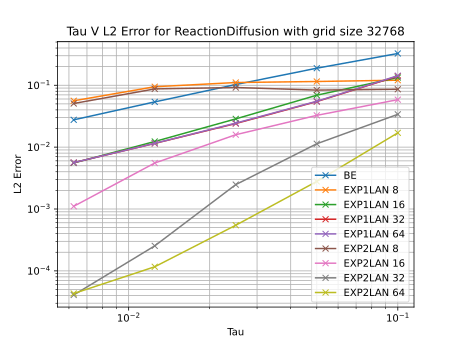
\includegraphics[width=1\textwidth]{Graphs/ReactionDiffusion/Tau V L2 Error for ReactionDiffusion with grid size 32768.png} % Change filename to your image
        \caption{$\tau$ vs $L_2$ with grid size 32768}
        \label{fig:ACtauE1024}
    \end{minipage}\hfill
\end{figure}
All methods appear to converge to the spacial discritisation error.
As above, we observe that the Krylov subspace must be sufficiently deep in order to be accurate.
In this example we can see that the second order method converges at a faster rate than the first order method as the slop for the second order method is steaper.
We also see that backwards Euler method has a higher error for a given value of $\tau$ for both methods.

Below as before we present the number of calls to the operator against the error.
\begin{figure}[H]
    \centering
    \begin{minipage}{0.49\textwidth}
        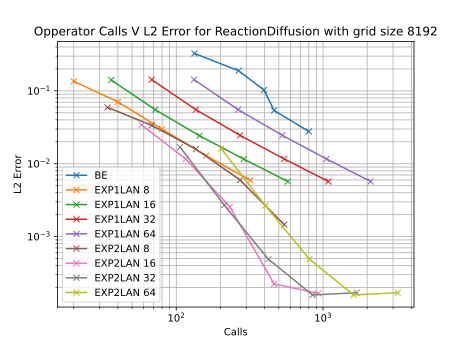
\includegraphics[width=1\textwidth]{Graphs/ReactionDiffusion/Operator Calls V Error for ReactionDiffusion with grid size 8192.png} % Change filename to your image
        \caption{Operator calls vs $L_2$ with grid size 1024}
        \label{fig:plot1}
    \end{minipage}\hfill
    \centering
    \begin{minipage}{0.49\textwidth}
        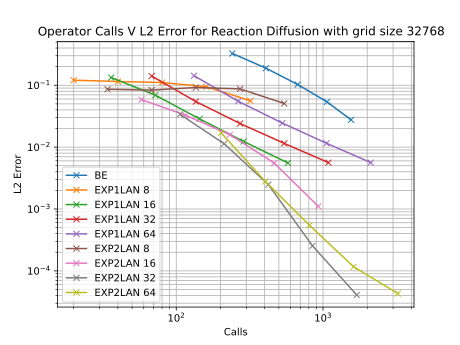
\includegraphics[width=1\textwidth]{Graphs/ReactionDiffusion/Operator Calls V Error for ReactionDiffusion with grid size 32768.png} % Change filename to your image
        \caption{Operator calls vs $L_2$ with grid size 2048}
        \label{fig:plot2}
    \end{minipage}\hfill
\end{figure}
Here we see that for all methods more operator calls are required to produce results with a smaller error.
The expoenential methods achieved a given error with fewer operator calls that the backwards Euler method.
The second order methods required fewer operator calls for a given error that the first order method, especially as the number of calls increased.


Here we present the experimental orders of convergence.
\begin{table}[H]
    \centering
    \begin{tabular}{| c | c | c |}
    \hline
    BE & EXP1LAN 64 & EXP2LAN 64 \\
    \hline
    0.7901637433430926 & 1.3717257454910614    & 2.608595189003896 \\
    0.8767440969959281 & 1.1734740319093697    & 2.3519399751018963 \\
    0.9320179419151513 & 1.0828183773958644   & 2.229913816965242\\
    0.963545660578168  & 1.03777329582159   & 1.4358363206568961 \\
    \hline
    \end{tabular}
    \caption{Experimental orders of convergence}
    \label{tab:reduced_data}
\end{table}

Now we observe the expected results, with the first order expoenential method converging at rate $1$ and the second order method converging at rate $2$.
\section{Conclusion}

This project has investigated the use of Krylov subspace methods, specifically Arnoldi and Lanczos alongside exponential integrators to provide numerical solutions to PDEs.
We have been able to demonstrate that this combination of methods can provide accurate solutions to PDEs with reduced computational cost relative to the backwards Euler method.
We have also begun to develop some error analysis of these methods in order to gain insight into how these Krylov methods affect the rate of convergence.
These methods show much promise for parabolic PDEs, especially phase boundary problems such as crystal growth.

Throughout this project, the size of the Krylov subspace played an important role in determining the accuracy of these results as well as performance demands.
Deeper Krylov subspaces yielded lower error, but had the downside of incurring a greater computational cost.
Further research could focus on how adapting the depth of this Krylov subspace dynamically during run time could improve performance such as with the KIOPS\cite{Gaudreault2018} method.

While much of our work focused on parabolic PDEs, we also showed that these methods may have possible application beyond the scope of parabolic PDEs.
These methods appeared effective for modeling the wave equation as well as showing potential in the modeling of atmospheric processes.
Further work could focus on applying these methods to a wider range of problems in order to properly understand the extent of their application, as well as how these methods apply to other spacial discretizations such as finite volume and finite difference.

\pagebreak

{\Huge \bf Bibliography}

\bibliographystyle{plain}
\bibliography{References.bib}
\bigskip

% These are examples of the book titles as they can be put in. 
% You can use different labeling methods, if you prefer, 
% e.g., just enumerating the items  as [1], [2], etc.,
% instead of making them [ATLAS], [B], etc.
% Or use bibtex



\end{document}
